\section{Frontend Frameworks}
\label{research:FrontendFramework}
\textbf{Sources:} \cite{AngularVsReact} \cite{AngularVsReact2021} \cite{ComparisonOtherFrameworks}
So far in my EPQ development journey I have been focusing on producing prototypes that highlight a specific aspect of my core idea (e.g. mapping nodes of thought). To achieve this I have produced many single page html pages which are then sent to the browser through my backend flask code. Any interaction between elements on the webpage have been linked by a complex web of JavaScript code which isn't maintainable as my project expands (despite my attempts to unify this previously) Whilst this has been very functional and easy for me to develop, as I start to incorporate more interconnected features such as multi-tab views and expand my current user preferences (settings, display scaling etc) I need to move forward to a more feature rich and standardised method.

Frontend frameworks enable developers to abstract away the complexities of handling multiple pages, elements and automatically refreshing visual signals when data is updated. For example, imagine a header on a website that displays the current number of times a button has been click, below the header is a simple button. Previously I would have had to write code for the button which directly interacts with the header to increment the value of the text when it is clicked, whilst this may seem fine imagine there was now 5000 textboxes scattered around which all showed the click count, you will see it gets very complicated quickly. This is one area my new development philosophy changes, instead of referencing each element the button now updates a global variable, my frontend framework then automatically updates each textbox which are simply bound to that global variable - much easier.


All framework would enable me to achieve this functionality nut I wanted to research my various options. From some brief searches I found three options that would fit my use case: React, Vue and Angular. On the surface all seemed to offer the same benefits but each had different way of achieving the same goals, below is a summary of my research and to the right are some sources I used:

React is a popular JavaScript library developed by Facebook for building user interfaces, primarily focusing on component-based architecture. It has a lightweight, flexible approach to UI development with fast updates and item rendering. React is known for its simplicity, strong community support, and a large ecosystem of third-party libraries. However, it requires additional tools and libraries for state management, routing, and other functionalities, making it more lightweight compared to other frameworks.

Vue is a progressive JavaScript framework that is easy to learn and integrate, making it a great choice for beginners and small to medium-sized projects such as mine. It combines the best features of React and Angular, offering a reactive data-binding system and a component-based approach while maintaining simplicity. Vue has a well-structured core library with optional ecosystem tools like Pinia for state management and Vue Router for navigation. Its has excellent documentation (widely praised in the industry)  and the ability to be gradually adopted into preexisting codebase making it a flexible and approachable option for developers first exploring frontend framework.

Angular, developed by Google, is a full-fledged front-end framework that provides a comprehensive solution for building large-scale applications. It follows a strict structure with built-in features like dependency injection, two-way data binding, and a powerful CLI (command line interface) tool for project scaffolding. Angular uses TypeScript (a subset of JavaScript which I already use), which adds static typing and better tooling support, making it suitable for enterprise applications. However, its steep learning curve and complexity can be challenging for developers, but it offers robustness and scalability for complex projects.

In conclusion I believe Vue is the best choice for my project. I can easily (and gradually) implement it into my project and it has a large (even if not as large as react) number of libraries which can add other common features. Whilst Vue doesn’t have close to the market share that React has (roughly half as seen below - source Stack Overflow survey (other entries removed for compactness), it is very popular in the smaller - medium developer scene and I have also found some other connections to it through my summer internship company (as documented in my diary) making it clear to be the tool I should learn to use

\begin{figure}[H]
    \centering
    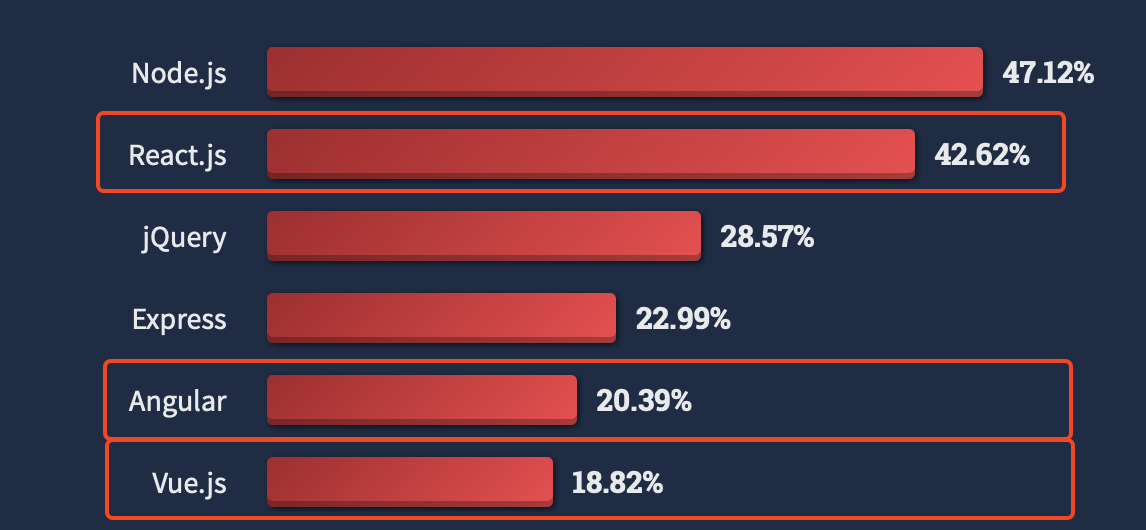
\includegraphics[width=0.6\textwidth]{Research/12_FrontendFramework/media/survey.png}
    \caption{Stack Overflow survey showing frontend framework usage \cite{StackOverflowDeveloper}}
\end{figure}

